% USEFUL LINKS:
% -------------
%
% - UiO LaTeX guides:          https://www.mn.uio.no/ifi/tjenester/it/hjelp/latex/
% - Mathematics:               https://en.wikibooks.org/wiki/LaTeX/Mathematics
% - Physics:                   https://ctan.uib.no/macros/latex/contrib/physics/physics.pdf
% - Basics of Tikz:            https://en.wikibooks.org/wiki/LaTeX/PGF/Tikz
% - All the colors!            https://en.wikibooks.org/wiki/LaTeX/Colors
% - How to make tables:        https://en.wikibooks.org/wiki/LaTeX/Tables
% - Code listing styles:       https://en.wikibooks.org/wiki/LaTeX/Source_Code_Listings
% - \includegraphics           https://en.wikibooks.org/wiki/LaTeX/Importing_Graphics
% - Learn more about figures:  https://en.wikibooks.org/wiki/LaTeX/Floats,_Figures_and_Captions
% - Automagic bibliography:    https://en.wikibooks.org/wiki/LaTeX/Bibliography_Management  (this one is kinda difficult the first time)
%
%                              (This document is of class "revtex4-1", the REVTeX Guide explains how the class works)
%   REVTeX Guide:              http://www.physics.csbsju.edu/370/papers/Journal_Style_Manuals/auguide4-1.pdf
%
%
% COMPILING THE .pdf FILE IN THE LINUX TERMINAL
% ---------------------------------------------
%
% [terminal]$ pdflatex report_example.tex
%
% Run the command twice, always.
%
% When using references, footnotes, etc. you should run the following chain of commands:
%
% [terminal]$ pdflatex report_example.tex
% [terminal]$ bibtex report_example
% [terminal]$ pdflatex report_example.tex
% [terminal]$ pdflatex report_example.tex
%
% This series of commands can of course be gathered into a single-line command:
% [terminal]$ pdflatex report_example.tex && bibtex report_example.aux && pdflatex report_example.tex && pdflatex report_example.tex
%
% ----------------------------------------------------



% \documentclass[english,notitlepage,reprint,nofootinbib]{revtex4-2}  % defines the basic parameters of the document
\documentclass[english,notitlepage,reprint,nofootinbib]{revtex4-2}  % defines the basic parameters of the document
% If you want a single-column, remove "reprint"

% Allows special characters (including æøå)
\usepackage[utf8]{inputenc}
% \usepackage[english]{babel}

% Note that you may need to download some of these packages manually, it depends on your setup.
% It may be usefult to download TeXMaker, because it includes a large library of the most common packages.

\usepackage{physics,amssymb}  % mathematical symbols (physics imports amsmath)
\include{amsmath}
\usepackage{graphicx}         % include graphics such as plots
\usepackage{xcolor}           % set colors
\usepackage{hyperref}         % automagic cross-referencing
\usepackage{listings}         % display code
\usepackage{subfigure}        % imports a lot of cool and useful figure commands
% \usepackage{float}
%\usepackage[section]{placeins}
\usepackage{algorithm}
\usepackage[noend]{algpseudocode}
\usepackage{subfigure}
\usepackage{tikz}
\usetikzlibrary{quantikz}
% defines the color of hyperref objects
% Blending two colors:  blue!80!black  =  80% blue and 20% black
\hypersetup{ % this is just my personal choice, feel free to change things
    colorlinks,
    linkcolor={red!50!black},
    citecolor={blue!50!black},
    urlcolor={blue!80!black}}


% ===========================================


\begin{document}

\title{FYS4150 - Project 1}  % self-explanatory
\author{Isak Cecil Onsager Rukan} % self-explanatory
\date{\today}                             % self-explanatory
\noaffiliation                            % ignore this, but keep it.
\maketitle
The one-dimensional Poisson can be written as 
\begin{align}
    -\frac{d^2u}{dx^2} = f(x),  \label{eq:Poisson}
\end{align}
where $f(x)$ is some known function. In this project we let \(x\in[0,1]\) and
\begin{align}
    f(x) = 100e^{-10x}, \label{eq:f_x}
\end{align}
together with the following boundary conditions
\begin{align}
    u(0)=0, \quad u(1)=0 \label{eq:boundary_condition}
\end{align}
\section{Problem 1}
% We will show that an analytic solution to \eqref{eq:Poisson} with \(f(x)\) given in \eqref{eq:f_x} is:
% \begin{align}
%     u(x) = 1 - (1-e^{-10})x - e^{-10x}.
% \end{align} 
Let $v(x)=d/dx u(x)$. Integrating \eqref{eq:Poisson} leads to 
\begin{align}
    -v(x) &= 100\int dxe^{-10x}
    \notag \\
    &= -10e^{-10x} + C,
\end{align}
which means that 
\begin{align}
    u(x) &= \int v(x) 
    \notag \\
    &= -e^{-10x} - Cx + D.
\end{align}
Here $C$ and $D$ are some constants which are determined by the boundary conditions in \eqref{eq:boundary_condition}. Concretely, \(u(0)=0\) leads to $D=1$ and then \(u(1)=0\) sets \(C=-(1-e^{-10})\). Hence,
\begin{align}
    u(x) = 1 - (1 - e^{-10x})x - e^{-10x}.
\end{align}
\section{Problem 2}
Using 
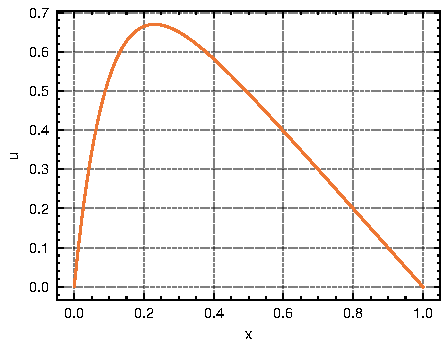
\includegraphics{Figs/problem2.pdf}

\onecolumngrid
% \bibliographystyle{apalike}
\bibliographystyle{unsrt}
\bibliography{ref}


\end{document}